\begin{enumerate}[resume]
    \item
    O programa abaixo realiza a cópia de um vetor de \textit{double words}, 
    convertendo-o de \textit{little endian} para \textit{big endian}.
    Complete o programa, indicando as instruções dos espaços em branco 
    (cada espaço deve ser preenchido com uma única instrução).

    \putNASM{Conversor de \textit{little endian} para \textit{big endian}.}{little_endian.asm}{little_endian}

    \item
    Para cada código C abaixo, escreva o equivalente em Assembly IA-32.
    Diretivas em C \textbf{devem} ser substituídas por diretivas equivalentes em IA-32.
    Use os registradores para as variáveis locais (com exceção de estruturas de dados)
    e seção de Dados ou BSS para as variáveis estáticas ou globais.
    \textbf{Deve-se} utilizar os endereçamentos corretos 
    para cada tipo de estrutura de dados.
    Não se preocupe pelo fato do programa principal em C ser uma função.
    \begin{itemize}
        \item [(a)] \putC{Vetor de 100 inteiros.}{vector_size_100.c}{vector_size_100}
        \item [(b)] \putC{Matriz indicadora de inteiros iguais.}{matrix_matching.c}{matrix_matching}
        \item [(c)] \putC{Soma dos elementos de um vetor.}{vector_sum.c}{vector_sum}
        \item [(d)] Não é permitido \asm{MUL} ou \asm{IMUL}.
                    \putC{Preenchimento de matriz 100x100.}{100x100_matrix.c}{100x100_martix}
        \item [(e)] Assuma que o usuário vai digitar um número de 0 a 9.
                    \putC{Soma com parâmetro na entrada do usuário.}{weird_sum.c}{weird_sum}
    \end{itemize}

    \item
    Escreva uma versão em C de cada uma das funções em Assembly IA-32
    (todas as funções em Assembly colocam o valor de retorno em EAX)
    seguindo as seguintes regras:
    \begin{enumerate}
        \item [(i)]
        todas as funções são compostas por uma \textbf{única instrução RETURN}
        sem criar variáveis locais,
        
        \item [(ii)]
        em nenhuma função em C pode ser utilizado deslocamento de bits 
        ($\ll$ ou $\gg$) e

        \item [(iii)]
        somente pode ser feita \textbf{uma única operação aritmética 
        e/ou uma única comparação} ($>$ ou $<$) nas funções em C.
    \end{enumerate}

    \begin{itemize}
        \item [(a)] \putC{foo1.}{foo1.asm}{foo1}
        \item [(b)] \putC{foo2.}{foo2.asm}{foo2}
        \item [(c)] \putC{foo3.}{foo3.asm}{foo3}
        \item [(d)] \putC{foo4.}{foo4.asm}{foo4}
    \end{itemize}

    \item   
    O código abaixo em C chama uma função em Assembly IA-32 que
    retorna o valor da multiplicação entre todos os elementos de um vetor.
    Escreva essa função em Assembly utilizando laços.

    \putC{Programa em C que chama função \asm{f4} em Assembly IA-32.}{f4.c}{f4}

    \item
    Considere um número em ponto flutuante baseado no formato da IEEE.
    O número é formado por 6 bits. 
    Um bit para o sinal, 
    os próximos três bits para o expoente,
    e os últimos dois bits para a mantissa.
    Como visto em sala de aula, o formato IEEE possui números normalizados,
    não normalizados, duas representações de zero, infinito e NaN.
    Assumindo que arrredondamentos são feitos utilizando
    o arredondamento ao inteiro mais infinito (\textit{ceil}),
    preencha a tabela abaixo (os lugares marcados com ``-'' não precisam ser preenchidos)
    nos campos \textit{binário}, \textit{mantissa}, \textit{expoente} e \textit{valor}.
    No campo \textit{binário}, deve-se colocar o binário do número completo,
    enquanto que nos outros campos deve-se colocar números decimais.
    Pode utilizar notação exponencial ($2^{512}$) ou fracionária (2$\frac{1}{3}$).
    Quando pede-se o maior/menor número, não deve ser considerando os  infinito.

    \begin{table}[H]
        \begin{tabular}{|l|l|l|l|l|}
            \hline
            \textbf{Descrição}  & 
            \textbf{Binário}    & 
            \textbf{Mantissa}   &
            \textbf{Expoente}   &
            \textbf{Valor decimal} \\\hline
            Menos zero & 100000 & 0 & $-2.0$ & $-0.0$ \\\hline
            Número positivo mais próximo a zero & & & & \\\hline
            Infinito negativo & & & & \\\hline
            Maior número normalizado & & & & \\\hline
            Menor número não-normalizado & & & & \\\hline
            $5.0 - 0.75$ & & & & \\\hline
            $4.0 + 3.0$ & & & & \\
            \hline
        \end{tabular}
        \label{tab:float 6 bits}
        \caption{Números a serem determinados em float de 6 bits}
    \end{table}

    \item
    Considere um número em ponto flutuante de 9 bits 
    baseado na representação IEEE (segue as regras para números normalizados,
    não normalizados, representação de 0, infinito e NaN), sendo que 
    existe 4 bits para o expoente e 4 bits para mantissa.
    Preencha a tabela abaixo.
    Se for necessário, arredonde para a fração mais próxima.
    No campo valor pode usar números fracionários (por exemplo, $\frac{3}{4}$)
    ou inteiros por potência de 2 (por exemplo $3\times2^{-3}$).

    \begin{table}[H]
        \begin{tabular}{|l|l|l|l|l|}
            \hline
            \textbf{Número}  & 
            \textbf{Valor}    & 
            \textbf{Bit sinal}   &
            \textbf{Bits expoente}   &
            \textbf{Bits mantissa} \\\hline
            Zero & 0.0 & 0 & 0000 & 0000 \\\hline
            Negativo mais próximo a zero & & & & \\\hline
            Maior positivo & & & & \\\hline
            n/a & $-5.0$ & & & \\\hline
            n/a & $1\frac{9}{16}\times2^{-2}$ & & & \\\hline
            Menos um & $-1.0$ & & & \\\hline
            O resultado de $4-1\frac{9}{16}$ & & & & \\
            \hline
        \end{tabular}
        \label{tab:float 9 bits}
        \caption{Números a serem determinados em float de 9 bits}
    \end{table}

    \item
    Considere um número em ponto flutuante baseado no formato da IEEE.
    O número é formado por 10 bits. 
    Um bit para o sinal, 
    os próximos cinco bits para o expoente,
    e os últimos quatro bits para a mantissa.
    Como visto em sala de aula, o formato IEEE possui números normalizados,
    não normalizados, duas representações de zero, infinito e NaN.
    Assumindo que arrredondamentos são feitos utilizando
    o arredondamento para o par mais próximo,
    preencha a tabela abaixo nos campos 
    \textit{binário}, \textit{mantissa}, \textit{expoente} e \textit{valor}.
    No campo \textit{binário}, deve-se colocar o binário do número completo,
    enquanto que nos outros campos deve-se colocar números decimais.
    Pode utilizar notação exponencial ($25^{12}$) ou fracionária (2$\frac{1}{3}$).
    Quando pede-se o maior/menor número, não deve ser considerando os  infinito.
    A base do expoente é 2.

    \begin{table}[H]
        \begin{tabular}{|l|l|l|l|l|}
            \hline
            \textbf{Descrição}  & 
            \textbf{Binário}    & 
            \textbf{Mantissa}   &
            \textbf{Expoente}   &
            \textbf{Valor decimal} \\\hline
            Número negativo mais próximo a zero & & & & \\\hline
            Maior número & & & & \\\hline
            Menor número não-normalizado & & & & \\\hline
            Menos um & & & & \\
            \hline
        \end{tabular}
        \label{tab:float 10 bits}
        \caption{Números a serem determinados em float de 10 bits}
    \end{table}

    \item
    O programa em C abaixo solicita ao usuário os valoers de uma matriz 10x10
    e depois calcula a soma dos elementos da diagonal principal.
    Altere o programa para uma versão em que o programa principal continua em C
    mas a função \asm{soma()} esteja em Assembly IA-32.
    A função deve calcular a soma dos elementos da diagonal principal,
    recebendo o ponteiro da matriz, o tamanho dela (NxN),
    e a variável de retorno da soma como parâmetros mediante a pilha.
    Mostre o código Assembly da função 
    e indique se é necessário fazer alguma alteração no código principal em C. 

    \putC{Programa C que chama função \asm{soma} em Assembly.}{soma.c}{soma}

    \item
    Considere o seguinte fragmento de código IA-32 
    obtido pelo comando \textbf{objdump}.
    Como pode ser visto, a função \asm{g()} é chamada pela função \asm{f()}.

    \putC{Resultado de um \asm{objdump}.}{objdump.asm}{objdump}

    \begin{itemize}
        \item [(a)]
        Quantos argumentos cada uma das funções \asm{f()} e \asm{g()} recebem?
        
        \item [(b)]
        Quando o CPU está a ponto de executar a instrução \asm{add} 
        no endereço \asm{0x0804838a} em \asm{g()}, mostre os valores na pilha, 
        preenchendo a tabela abaixo.
        \begin{figure}[H]\centering
            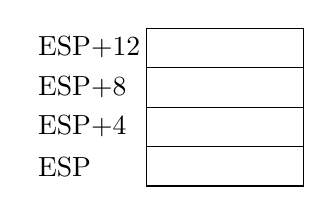
\begin{tikzpicture}[scale=.5]
                \draw
                    (0,0) rectangle (4,4)
                    (0,0) --++ (4,0)
                    (0,1) --++ (4,0)
                    (0,2) --++ (4,0) 
                    (0,3) --++ (4,0)
                ;
                \draw
                (-3, 3) node [above right] {\asm{ESP+12}} ++ (0, -1)
                        node [above right] {\asm{ESP+8}}  ++ (0, -1)
                        node [above right] {\asm{ESP+4}}  ++ (0, -1)
                        node [above right] {\asm{ESP}}
                ;
            \end{tikzpicture}
        \end{figure}
    \end{itemize}

    \item
    Escreva o seguinte código em Assembly IA-32.
    Para isso é permitido o uso da bibiloteca io.mac
    para ler e escrever strings (PutStr, GetStr).
    O programa em Assembly deve mostrar 
    todas as mensagens indicadas no programa em C.
    Deve manter os ponteiros para arquivo em memória.
    Assuma que ambos arquivos, entrada e saída, já existem 
    (o arquivo de saída existe, mas está vazio).

    \putC{Programa em C que lê um arquivo de entrada e escreve no de saída.}
         {files.c}{files}

    \item
    Faça um programa em Assembly IA-32
    que multiplique duas matrizes 5x5 de inteiros.
    O programa deve primeiro fazer um laço 
    para preencher a primeira matriz a ser digitada pelo usuário.
    Depois deve fazer um laço 
    para preencher a segunda matriz digitada pelo usuário.
    Em seguida, deve multiplicar as duas matrizes
    e salvar o resultado em outra matriz.
    Utilize o endereçamento correto para matrizes.
    Os labals das matrizes devem ser declarados no SECTION BSS.
    Não é necessário imprimir mensagens para o usuário,
    nem mostrar o resultado final.




\end{enumerate}
